\chapter{Overview}\label{ch:overview}

In this document we introduce the Metrics component of the Test and Evaluation Framework (TEF) for Agent-based evaluation \textit{only.} For this preliminary information release, we focus on a high level overview of the system, followed by a brief introduction to the types of syllabi and metrics which are expected, and end with how to get started with the code. Stay tuned for more details in each of these areas!

\section*{Core Capabilities Review}
\label{sec:core_capabilities}

We remind readers that the purpose of the metrics discussed in this document are to determine whether a system exhibits the Core Capabilities of Lifelong Learning. These metrics may be slightly different from those which might assess a traditional learner. We invite our audience to review the five Core Capabilities whose definitions are below, and refer readers to the BAA for more details.\\%\footnote{DARPA L2M Broad Agency Announcement (April 12 2017)}
\\
\textbf{1. Continual Learning}\\

Ability to handle, or adapt to, changing input distributions (or noise characteristics) within a single task. For an agent-based system, this means that the state transition matrix and reward function are substantively unchanged, while aspects of the environment may change.\\
\\
\textbf{2. Adapting to New Tasks}\\

Ability to learn new tasks, without losing knowledge of already-learned tasks. If possible, system should exploit similarities between old and new tasks to improve its learning performance on new tasks. For an agent-based system, this means substantial changes to the state transition matrix or reward function.\\
\\
\textbf{3. Selective Plasticity}\\

Ability to process the same input differently depending on task (or goal). Relatedly, the ability to be sensitive to different features of the input depending on task. Note the focus on processing rather than learning per se.\\
\\
\textbf{4. Goal-Driven Perception}\\

Ability to incorporate system and task-level constraints (e.g., overall memory use, relative importance of tasks) into the training process.\\
\\
\textbf{5. Safety}\\

Ability to incorporate explicit (failsafe) safety constraints into system performance; Ability to detect differences between training and test environments (e.g., anomalous inputs, distributional shifts), quantify the resulting uncertainty in system output, alert a human operator (with details of difference if possible), and safely handle the anomalous situation where possible.

\section*{Measurement Framework Architecture}

\textit{Overview}
\\

The Test and Evaluation Framework (TEF) uses the information contained in a syllabus to produce a sequence of episodes for an agent learner. Figure~\ref{fig:systemlayout} depicts a high level overview of the TEF system. The syllabus passes the sequence of episodes to the TEF which sets up an environment and makes it available to the 

\begin{figure}[h]
	\centering
	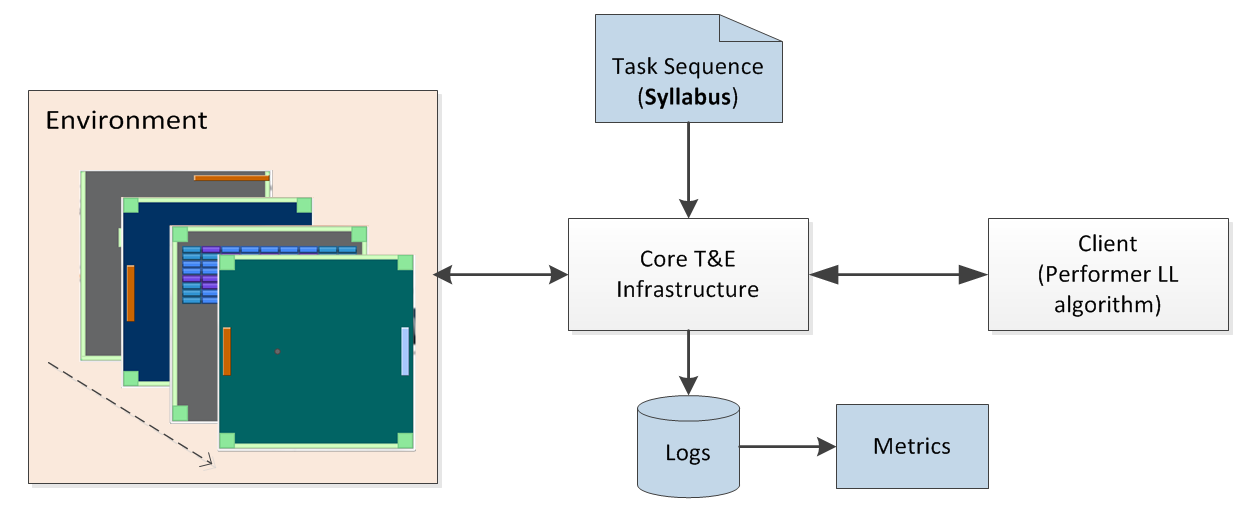
\includegraphics[width=0.85\columnwidth]{sections/figs/metrics_diagram.png}
	\caption{This figure describes the production of Metrics from Log files outputted by the Core Test and Evaluation Framework.}
	\label{fig:systemlayout}
\end{figure}

Figure~\ref{fig:syllabus} shows an example syllabus which would evaluate the Continual Learning Core Capability. You can see that only one task is exercised throughout the syllabus, but parameter variation - agent\_pos and agent\_dir are paramters for this task - is contained throughout the syllabus. Additionally, later Test phases contain previously trained parameters, allowing for a maintenance calculation. Unless otherwise noted, an instance of a syllabus is considered a Lifetime, and metrics are computed on an Agent's performance on episodes within a syllabus.

\pagebreak
\begin{figure}[h]
	\centering
	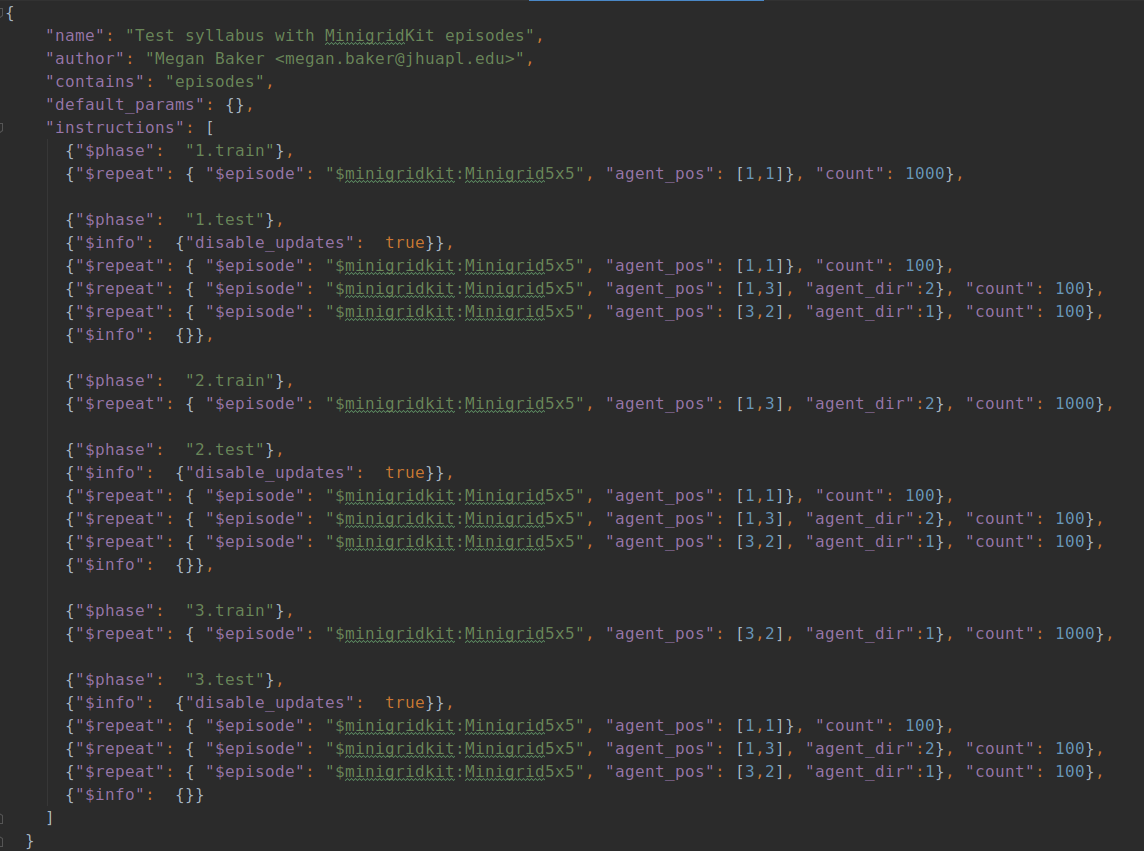
\includegraphics[width=0.75\columnwidth]{sections/figs/syllabus.png}
	\caption{An example syllabus.}
	\label{fig:syllabus}
\end{figure}



When an Agent performs episodes from the syllabus, the TEF will automatically generate logs which are saved in a tab separated file like shown in Figure~\ref{fig:logfile}. Then, the Metrics code scrapes these logs and extracts the relevant information to produce a set of scores for each metric used to evaluate the Core Capabilty being tested.\\



\begin{figure}[h]
	\centering
	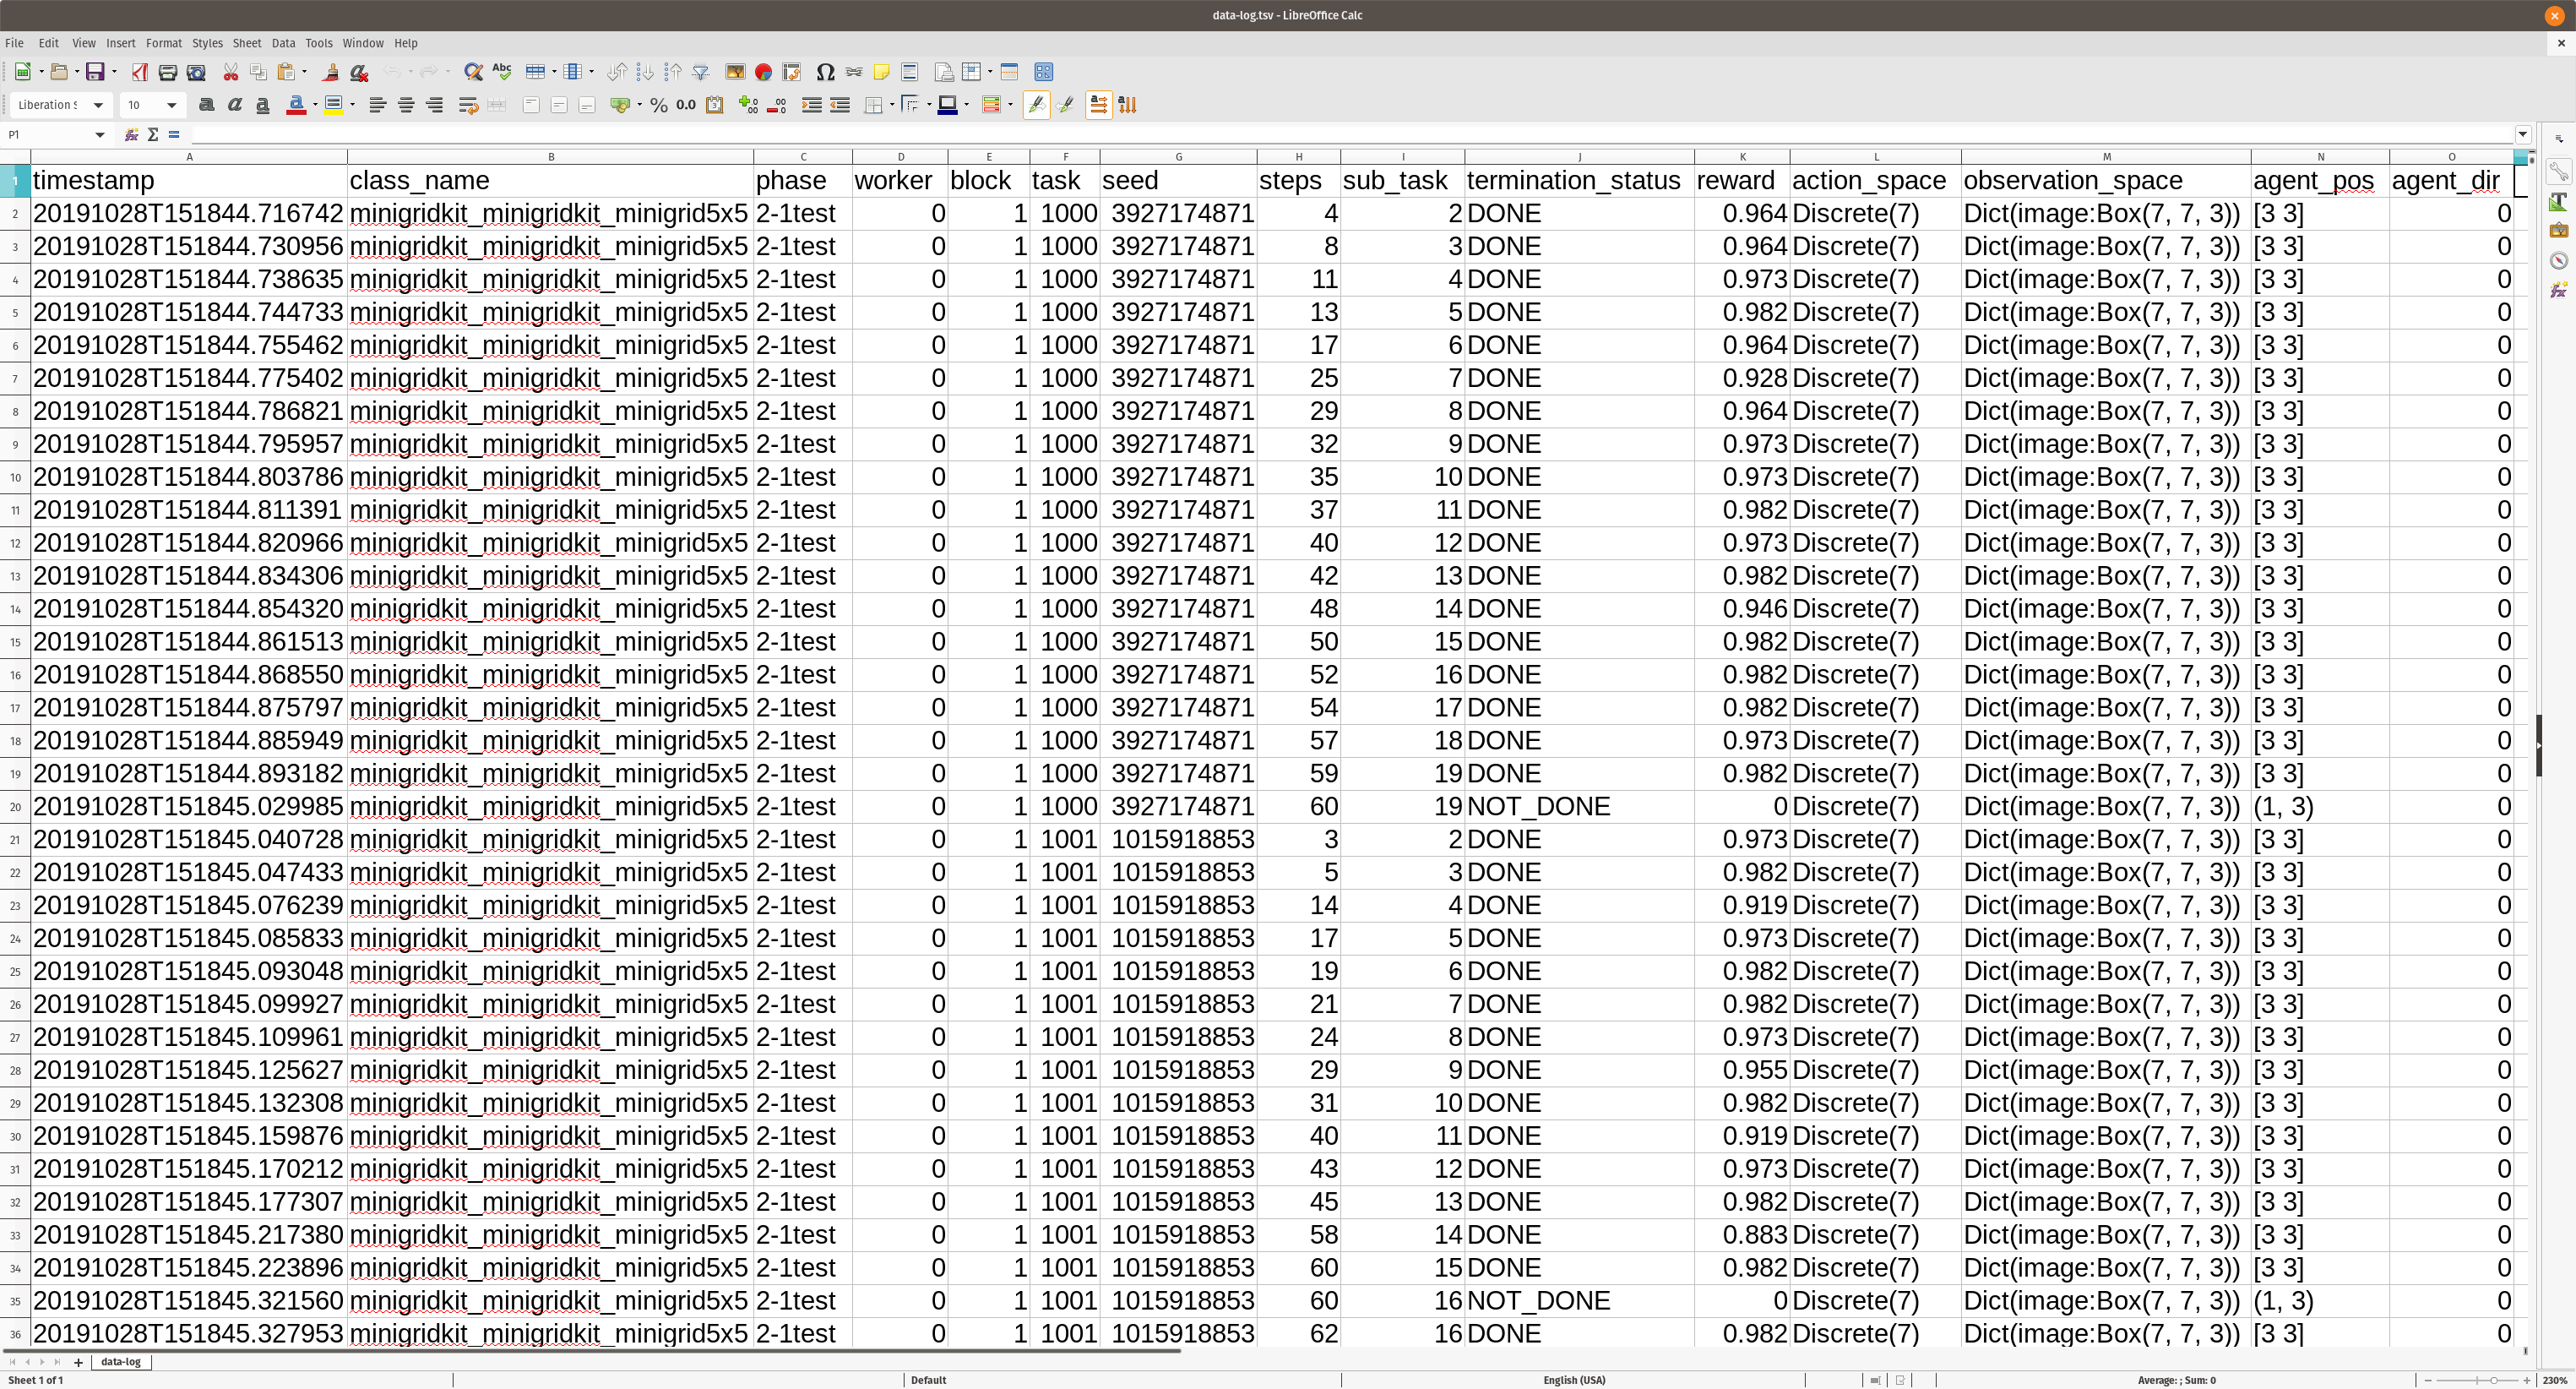
\includegraphics[width=0.75\textwidth]{sections/figs/log_file.png}
	\caption{An example log file.}
	\label{fig:logfile}
\end{figure}


\iffalse

For the purpose of this initial development, we chose to focus our attention on the first two Core Capabilities; Continual Learning and Adapting to New Tasks. 

\section{Terminology}

\\
Task: A single abstract capability (or skill) that a performer system must learn\\
Episode: A concrete instance of a task\\
Syllabus: A sequence of episodes\\
Learning Lifetime: One syllabus or multiple syllabi in sequence\\
\\
\textit{Metric Specific Terms for Syllabus Design}\\
Phase: A subcomponent of a syllabus during which either training or evaluation takes place\\
Block: A unique combination of task and parameters. It is a subcomponent of phase that is automatically assigned by the logging code and does not need to be annotated by the syllabus designer.\\

\textit{Key Concepts}

\fi

% footnote example : \footnote{\url{http://www.es.ele.tue.nl/cvpm18/}}
% citation example : \cite{verkruysse2008remote} 
%\subsection*{Example subsection}
%Subsection related work.
